%%=============================================================================
%% CI/CD pipeline
%%=============================================================================

\chapter{\IfLanguageName{dutch}{CI/CD pipeline}{CI/CD pipeline}}
\label{ch:cicd-pipeline}
Dit hoofdstuk zal een Continuous Integration en Continuous Delivery pipeline in detail bekijken. Binnen een CI/CD pipeline zijn er verschillende lagen die elkaar aanvullen en opvolgen. Deze worden hier kort besproken, omdat dit een essentieel onderdeel is van de thesis. De voordelen, alsook de nadelen, van zo een pipeline worden ook aangehaald. Om de algemene voor- en nadelen te vinden wordt er teruggegrepen naar de literatuur. Er is namelijk al enorm veel geschreven over een CI/CD pipeline en wat de voor- en nadelen kunnen zijn. De toegevoegde waarden en de schaduwzijden van een CI/CD pipeline voor Amista worden aangeduid door Pieter-Jan Deraedt, CTO bij Amista.

    \section{Continuous Integration en Continuous Delivery pipeline}
    De pipeline stelt het proces van de verschillende workflows voor die reeds in deze thesis besproken zijn. Het is een samentrekking tussen het proces van Continuous Integration en Continuous Delivery waarbij alles automatisch wordt aangestuurd. In onderstaande figuur \ref{cicd-pipeline} is te zien hoe een pipeline eruit ziet waar alle basislagen aan bod komen en integreren met elkaar.
    Alles begint bij de developer die een verandering in de code aanbrengt en deze commit naar de version control repository waar de build scheduler toegang toe heeft. De build scheduler merkt op zijn beurt de commit en begint aan zijn taak: het builden van de code. Voor deze stap zorgt de build scheduler ervoor dat de unit testen uitgevoerd zijn alvorens de build begint. Eens de testen en de build slagen is het de taak om de automatische build tests uit te voeren en de code uitvoerig te testen of deze klaar is voor productie. Dit kan op een realistische testomgeving gebeuren of de code wordt door iemand anders nagekeken of deze voldoet aan alle kwaliteitseisen. Eens de code door de testen raakt wordt deze klaar gemaakt voor productie door deze naar de stage fase te brengen. Eens de code zich in de stage fase bevindt kan deze manueel worden gedeployed om naar de klant te brengen.
    
    \begin{figure}	
        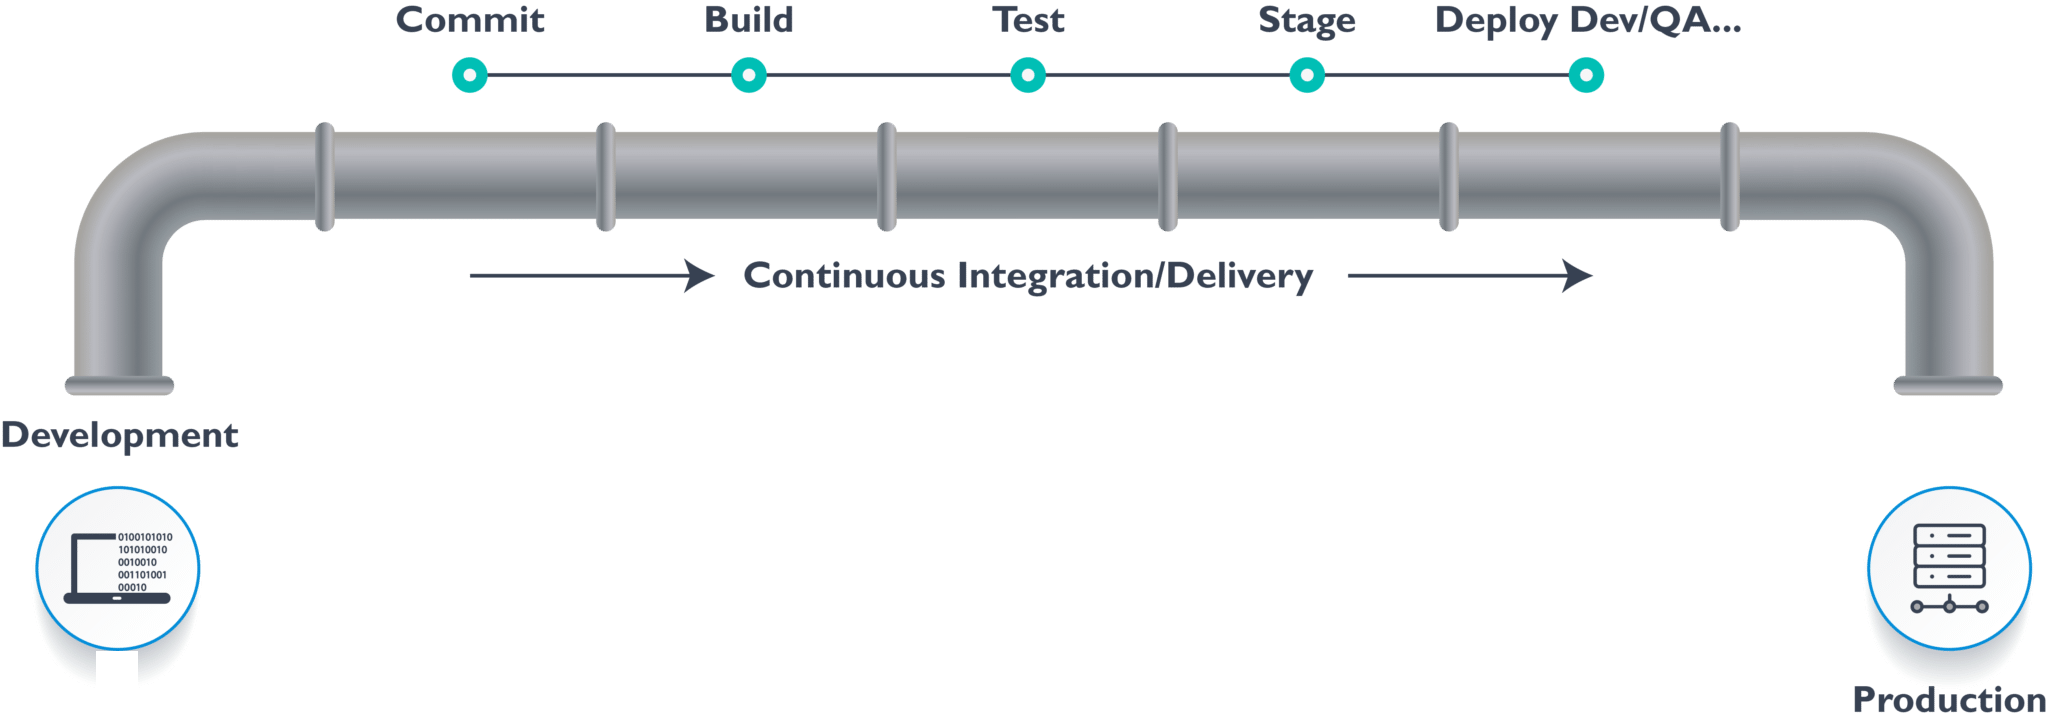
\includegraphics[scale=0.2]{cicd-pipeline}
        \caption{Continuous Integration en Continuous Delivery pipeline ~\autocite{Tuli2018}} \label{cicd-pipeline}
    \end{figure}
    
    \section{Lagen binnen een CI/CD pipeline en beschikbare tools}
    De CI/CD pipeline bestaat uit verschillende lagen die naadloos met elkaar moeten samenwerken om het beste resultaat te bekomen. De verschillende taken en beschikbare tools van elke laag worden besproken.
    
        \subsection{Source Control System}
        \label{subsec:source-control-systeem}
        Dit systeem houdt alle veranderingen bij aan de code en zal de veranderingen ook beheren zodat ze niet overlappen. Het laat toe dat meerdere developers tegelijk aan - soms dezelfde - code werken. Een source control systeem houdt dan de veranderingen bij wat elke developer gedaan heeft. Een best practice is dat er één stabiele versie van de software bestaat, meestal master genoemd.\\
        Een gangbare praktijk binnen dit systeem is het maken van branches. Hier wordt een kopie gemaakt van de stabiele master, waardoor men wat kan knoeien in de branch zonder de master te beschadigen. Als men overtuigd is van de kwaliteiten dat men op een branch gemaakt heeft kan men de branch 'mergen' in de master. Deze techniek wordt ook wel 'revision control' of 'version control' genoemd ~\autocite{Skelton2014} en ~\autocite{Riti2018}.
        Voorbeelden van zo een source control system zijn Git, CVS (Concurrent Version System), Subversion en Mercurial.
        
        \subsection{Hosted Version Control Services}
        Wordt ook wel Code Repository Server genoemd. Hier wordt de software van het source control system opgeslagen. Dit kan op een interne server opgeslagen worden, of op een externe die door bedrijven aangeboden wordt. Dit maakt het makkelijker voor developers om samen te werken en dezelfde bron te gebruiken. Deze stap is ook crusiaal om een goede Continuous Integration te voorzien.
        Voorbeelden van Repository Management Services zijn: GitHub, BitBucket, GitLab en Coding zijn veruit de populairste op de markt.
        
        \subsection{Build Scheduler}
        Een Build Scheduler kan ook wel een Continuous Integration Server genoemd worden.
        Dit zorgt ervoor dat - telkens wanneer er code gecommit wordt - de stappen in de pipeline worden uitgevoerd. De taken van de build scheduler zijn: 
        \begin{itemize}
            \item De nieuwe code ophalen van de Repository Server en deze samenvoegen met de oude code
            \item De testen uitvoeren
            \item Het builden van de software
            \item Feedback geven aan de developer over voorgaande stappen
        \end{itemize}
        Deze taken kunnen ook door een script volbracht worden, maar het is belangrijk dat deze taken automatisch gebeuren telkens er code gecommit wordt naar de repository manager ~\autocite{Riti2018}.
    
        In het hoofdstuk \ref{ch:methodologie} worden de meest populaire build schedulers van vandaag met elkaar vergeleken. Naast Jenkins, Circle CI, Bamboo en Travis CI zijn er nog andere build schedulers op de markt die gebruikt kunnen worden: Team City, Gitlab CI, CodeShip en nog enkele tientallen.
        
        
        \subsection{Artifact Repository Manager}
        Als laatste zijn de Artifact Repository Managers aan de beurt. Deze repository manager houdt alles bij wat nodig is om de applicatie te deployen, zoals:
        \begin{itemize}
            \item Gecomprimeerde applicatie code
            \item Code in verband met de infrastructuur
            \item Images van virtuele machines
            \item Configuratie data
        \end{itemize}
        Deze tool houdt alle geschiedenis bij van de bovenstaande files. Zoals eerder vermeld kan men vanaf hier de software (automatisch) deployen. Dit is de allerlaatste fase in de CI/CD pipeline ~\autocite{Skelton2014}.
        Sonatype Nexus en Archiva zijn dan weer voorbeelden van tools die gebruikt worden als artifact repository manager, deze houden bij wijze van spreken de code bij die klaar is om te deployen. 
    
    \section{Voordelen}
    \begin{itemize}
        \item Maak de applicatie die de klant wil. Het grootste probleem bij het falen van projecten ligt nog altijd bij het te grote verschil tussen de gemaakte applicatie en hetgeen de klant voor ogen had. Elke persoon die met IT bezig is weet dat de klant heel vaak niet weet wat hij wil. Dit is zeer gevaarlijk wanneer er grote projecten moeten afgeleverd worden en de klant al 10 keer van idee veranderd is tegen de datum van oplevering. Mede dankzij een combinatie van Agile en CI/CD is het makkelijker om een minimale hoeveelheid aan code te schrijven, dit aan de klant te tonen, feedback te krijgen en erop verder te bouwen. CI/CD komt hier echt tot zijn recht vanwege de makkelijkheid om voort te bouwen op geschreven software en tevens de kwaliteit van voorgaande geschreven code niet te verliezen. Dit is de ideale combinatie om samen met de klant tot een gewild en bruikbaar product te komen ~\autocite{Humble2012}.
        \item Wanneer men de principes van CI/CD volgt en minstens één keer per dag code commit naar de main repository verkleint dit de kans op grote bugs. Bij het pushen van kleine stukjes code en de onmiddellijke feedback die volgt door de build scheduler, weet het team of de developer dat er iets mis is met het kleine stukje code die hij probeerde te pushen richting repository. Het is op deze manier veel makkelijker om de fout eruit te halen dan wanneer de developer moet zoeken in code die hij weken geleden geschreven heeft. ~\autocite{Fowler2006}.
        \item Bij het niet krijgen van feedback over de kwaliteit kan het gebeuren dat de developer voortbouwt op foutieve code. Door het onmiddellijk krijgen van feedback kan er veel tijd bespaard worden.
        \item Wanneer de developer een fout heeft ontdekt vlak na het pushen van de code zal hij die fout, hoogst waarschijnlijk, niet meer opnieuw maken. Dit zal veel tijd besparen tijdens verdere implementatie.
        \item In de meeste omgevingen met een CI/CD pipeline is het niet nodig om een Quality Assurance team (QA team dat waakt over de kwaliteit van de software) te hebben om de testen uit te voeren, wat de kosten doet dalen.
        \item Het risico op downtime van een applicatie verkleind door de vele testen die automatisch gerund worden alvorens de aanpassing naar buiten wordt gebracht. Dit is wel onder de voorwaarde dat de testen in een soortgelijke omgeving als de echte applicatie worden getest en dat de testen aan alle kwaliteitseisen voldoen om de applicatie werkende te houden.
        \item De stress die komt kijken bij een release kan achterwege gelaten worden. Door continu kleine aanpassingen door te voeren, die aan alle kwaliteitseisen voldoen eens ze door alle testen raken, zal er minder stress bij komen kijken. Dit is een heel groot voordeel voor iedereen die iets met de applicatie te maken heeft. Wanneer een team minder stress ervaart zal het ook minder fouten maken en de productiviteit ten goede komen.
        \item Bij een grote release is er soms ook een team van wacht die problemen, wanneer ze opduiken, kunnen oplossen. Bij een CI/CD pipeline is het niet nodig om schrik te hebben voor problemen omdat de software uitvoerig getest geweest is alvorens live te gaan.
    \end{itemize}
    
    \section{Nadelen}
    Het vergt echter wat inspanningen om een Continuous Integration en Continuous Delivery pipeline op te zetten. De inspanningen moeten door heel het bedrijf geleverd worden.
    \begin{itemize}
        \item Er zal heel wat werk kruipen in het opzetten van een CI/CD pipeline. Dit gaat gepaard met werkuren, die geld kosten.
        \item De developers moeten zich ervan bewust zijn dat het enorm belangrijk is om op regelmatige basis en met kleine werkende aanpassingen de code naar de repository te sturen. Dit kan een aanpassing vergen om op deze manier te werk te gaan.
        \item Er kruipt heel wat tijd in het schrijven van goede testen die de applicatie op alle vlakken voldoende test.
        \item De geschreven testen moeten ook zeer goed onderhouden worden. Elke nieuwe functionaliteit moet uitvoerig getest worden zonder de vorige functionaliteiten uit het oog te verliezen.
        \item Wanneer het team nog nooit met een CI/CD tool heeft gewerkt vraagt dit ook een aanpassing dat vaak gepaard gaat met een training.
        \item Wanneer gekozen wordt om de code op een lokale server te runnen moet deze server ook onderhouden worden om veilig te blijven functioneren.
        \item Er komen nieuwe technologieën kijken bij het opzetten van een CI/CD pipeline. Sommige tools moeten betaald worden alvorens te kunnen gebruiken. 
    \end{itemize}